% ----------------------------------------------------------
% Metodologia
% ----------------------------------------------------------
\chapter{Metodologia}\label{cap:metodologia}
% ----------------------------------------------------------

% ----------------------------------------------------------
\section{Métodos e Etapas}\label{sec:metodos-etapas}
% ----------------------------------------------------------

O projeto e desenvolvimento do Peacon foi dividido em três etapas. A primeira foi o levantamento bibliográfico relacionado ao tema, na qual foram realizadas buscas relacionadas aos assuntos: \textit{Raspberry Pi}, comunicação via \textit{Bluetooth Low Energy}, \textit{beacons}. Concomitantemente foi realizado o estudo prático das tecnologias, levando em conta suas capacidades, limitações, e aplicações.

A segunda etapa foi projetar o Peacon baseado na análise do levantamento bibliográfico, assim como a definição de sua estrutura. Essa etapa foi necessária para facilitar e agilizar a implementação e testes dos componentes nas próximas etapas, definindo assim um escopo inicial de funcionalidades que o sistema terá, assim como outras tarefas a serem realizadas. O processo está detalhado no \autoref{cap:desenvolvimento}.

A terceira etapa foi a implementação e testes do Peacon. As funcionalidades foram divididas em módulos para facilitar os testes e detectar possíveis erros e \textit{bugs}.

% ----------------------------------------------------------
\section{Materiais Utilizados}\label{sec:materiais-utilizados}
% ----------------------------------------------------------

% ---
\subsection{Raspberry Pi e Acessórios}\label{sec:rpi-acessorios}
% ---

A versão do Raspberry Pi escolhida para o projeto foi a 2 Modelo B, por ter mais processamento e mais memória RAM (\autoref{fig:rpi2-utilizado}), conforme informado na \autoref{sec:raspberry-pi}.

É necessário o uso de um adaptador \textit{WiFi} para conexão a internet sem necessidade de cabo \textit{Ethernet} e também um adaptador Bluetooth 4.0 com suporte a \textit{BLE} para fazer a busca dos pacotes \textit{beacon}. Os modelos de adaptadores usados foram Orico BTA-406 (bluetooth) e EDUP N8508GS (\textit{WiFi}), conforme \autoref{fig:adaptadores}.

O sistema operacional executado no RPi foi instalado em um cartão microSD, com no mínimo 4 GB de espaço. O cartão utilizado nesse projeto foi um SanDisk Ultra Class 10 de 8 GB. 

O sistema utilizado foi o Raspbian Wheezy. Durante o desenvolvimento do projeto, a versão Raspbian Jessie foi lançada, com inúmeras melhorias, porém preferiu-se permanecer na versão Wheezy para evitar possíveis incompatibilidades com os softwares utilizados.

Na \autoref{sec:rpi-tecnologia} aborda-se como o \textit{RPi} funciona na prática, como foi utilizado para esse projeto e como suas capacidades foram aproveitadas.

\begin{figure}[htb]
	\label{teste}
	\centering
 	\begin{minipage}{0.47\textwidth}
		\centering
		\caption{\label{fig:rpi2-utilizado}\textit{RPi} 2 modelo B utilizado nesse projeto.}
		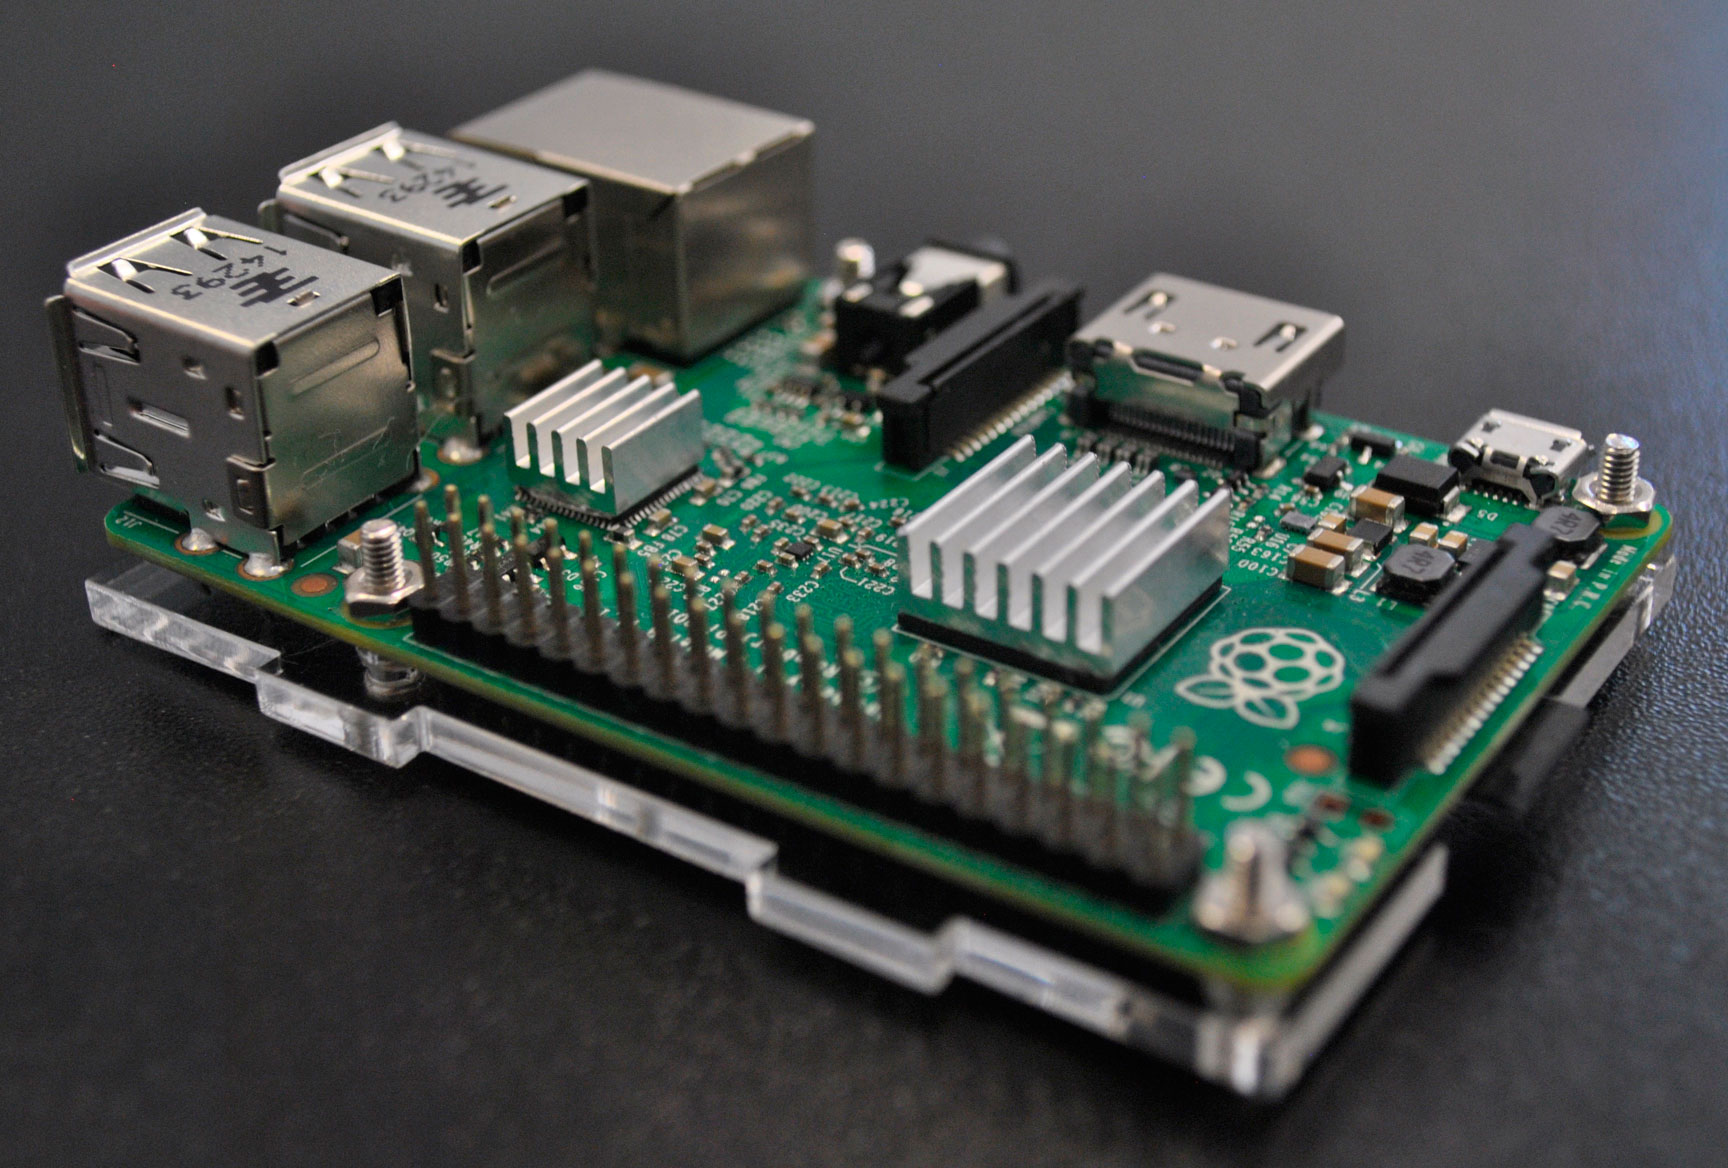
\includegraphics[width=1\textwidth]{img/rpi2.jpg}
		\legend{Fonte: elaborado pelo autor}
	\end{minipage}
	\hfill
	\begin{minipage}{0.45\textwidth}
		\centering
		\caption{\label{fig:adaptadores}Orico BTA-406 a esquerda e EDUP N8508GS a direita.}
		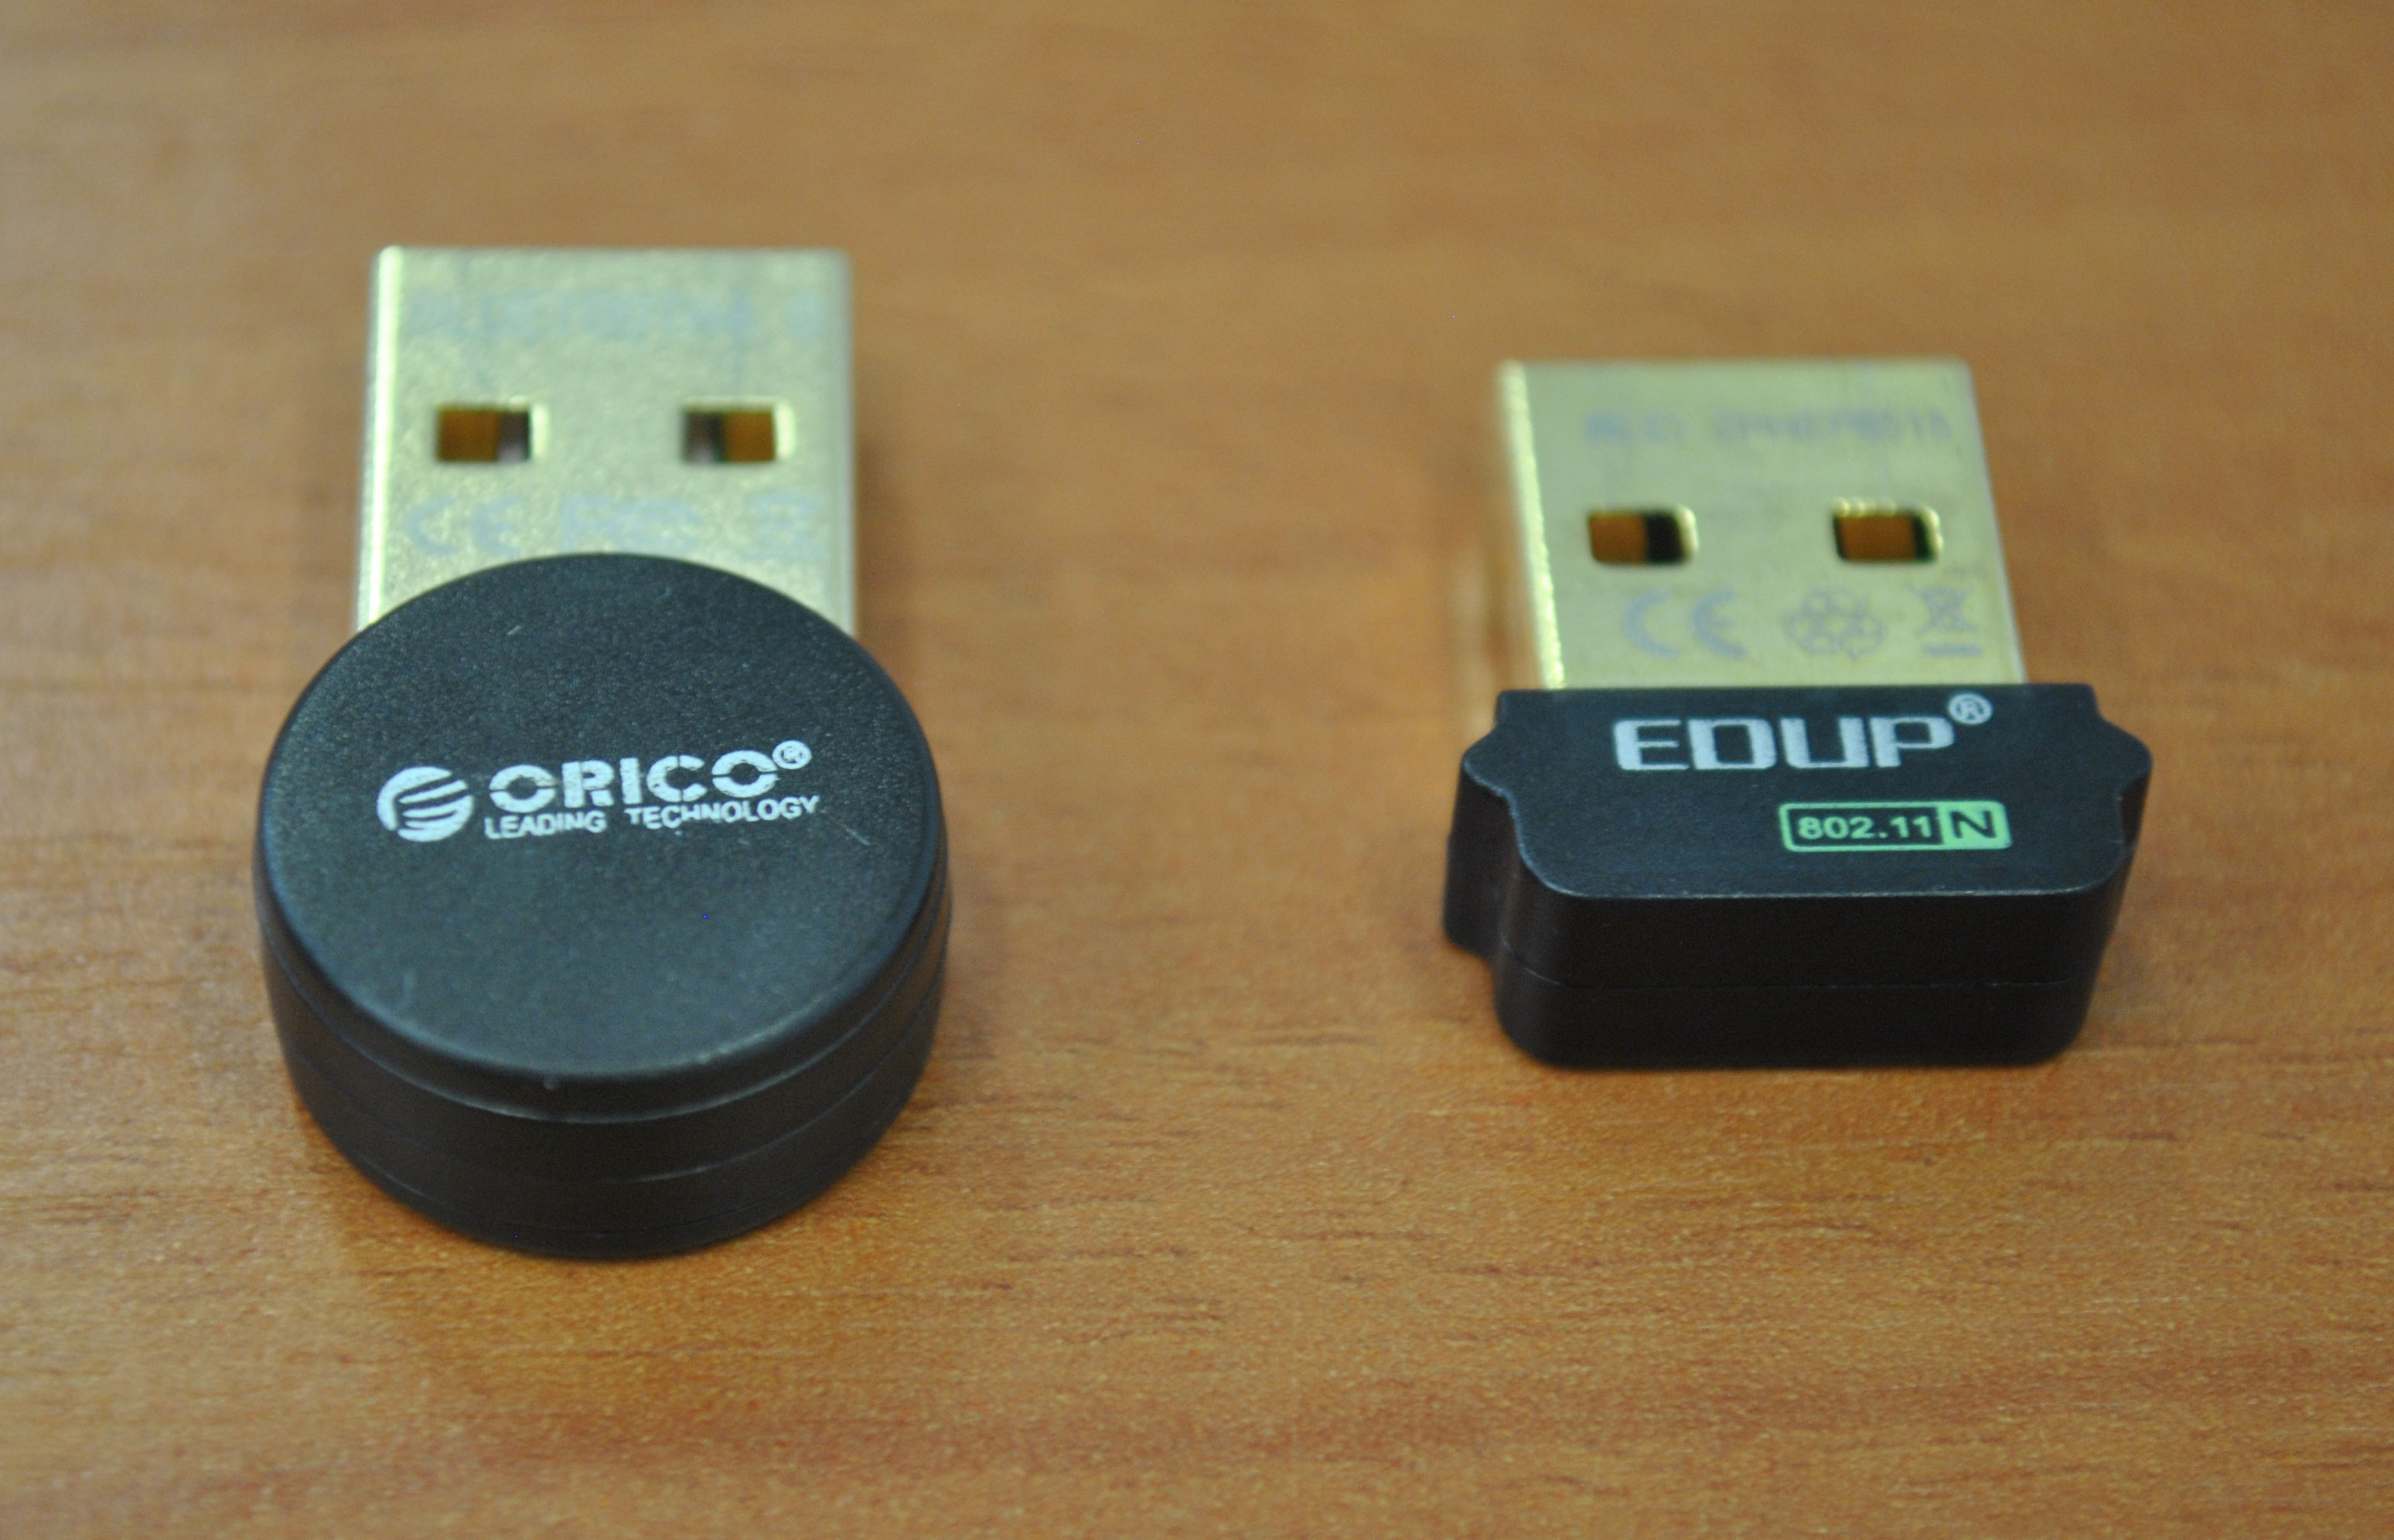
\includegraphics[width=1\textwidth]{img/adaptadores.jpg}
		\legend{Fonte: elaborado pelo autor}
	\end{minipage}
\end{figure}

% ---
\subsection{Computadores e Softwares}\label{sec:comp-softwares}
% ---

A conexão com o \textit{RPi} foi realizada utilizando \textit{SSH}\footnote{\textit{Secure Shell}}, sem necessidade de monitor e teclado. O computador utilizado no projeto foi um MacBook Pro com sistema Mac OS X 10.10, posteriormente atualizado para 10.11. 

Nesse sistema o uso de \textit{SSH} é simples, basta abrir o aplicativo Terminal e utilizar o comando "\textit{ssh usuario@computador}", conforme \autoref{fig:ex-terminal}. Esse tipo de abordagem é bastante utilizada para conexão a servidores na nuvem, para executar comandos, softwares, entre outros.

\begin{figure}[htb]
	\caption{\label{fig:ex-terminal}Conexão com o \textit{RPi} via \textit{SSH}.}
	\begin{center}
		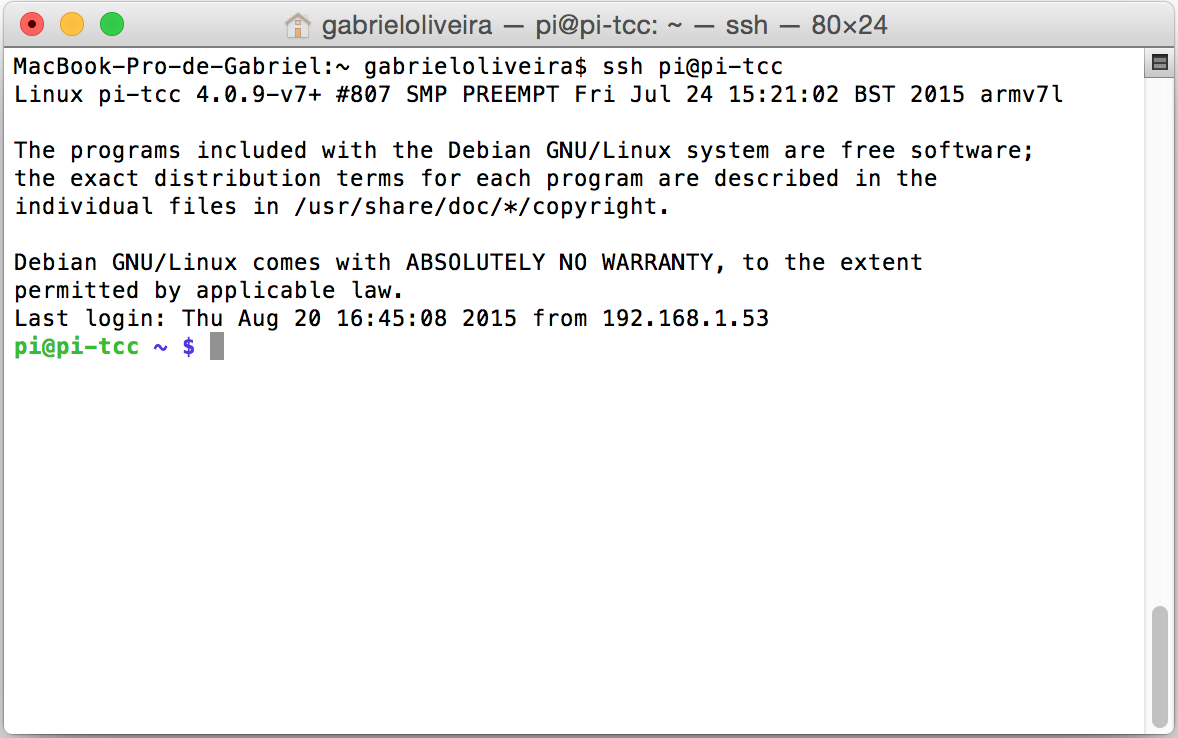
\includegraphics[width=0.6\textwidth]{img/terminal-pi.png}
	\end{center}
	\legend{Fonte: elaborado pelo autor}
\end{figure}

% ---
\subsection{Smartphones e Tablets}\label{sec:smartphone-tablets}
% ---

Foram utilizados o smartphone Moto Maxx com sistema Android 5.0.1 e o tablet iPad mini Retina com sistema iOS 8.4 mostrados na \autoref{fig:motomaxx-ipad}. 

O aplicativo utilizado em ambos foi o \textit{Locate Beacon} da \textit{Radius Networks}, que nos permite identificar os \textit{beacons} e também simular um, para realizar os testes com diferentes tipos, podendo alterar os valores de UUID, Major, Minor e potência de transmissão. 

\begin{figure}[htb]
	\caption{\label{fig:motomaxx-ipad}Moto Maxx (esquerda) e iPad Mini (direita).}
	\begin{center}
		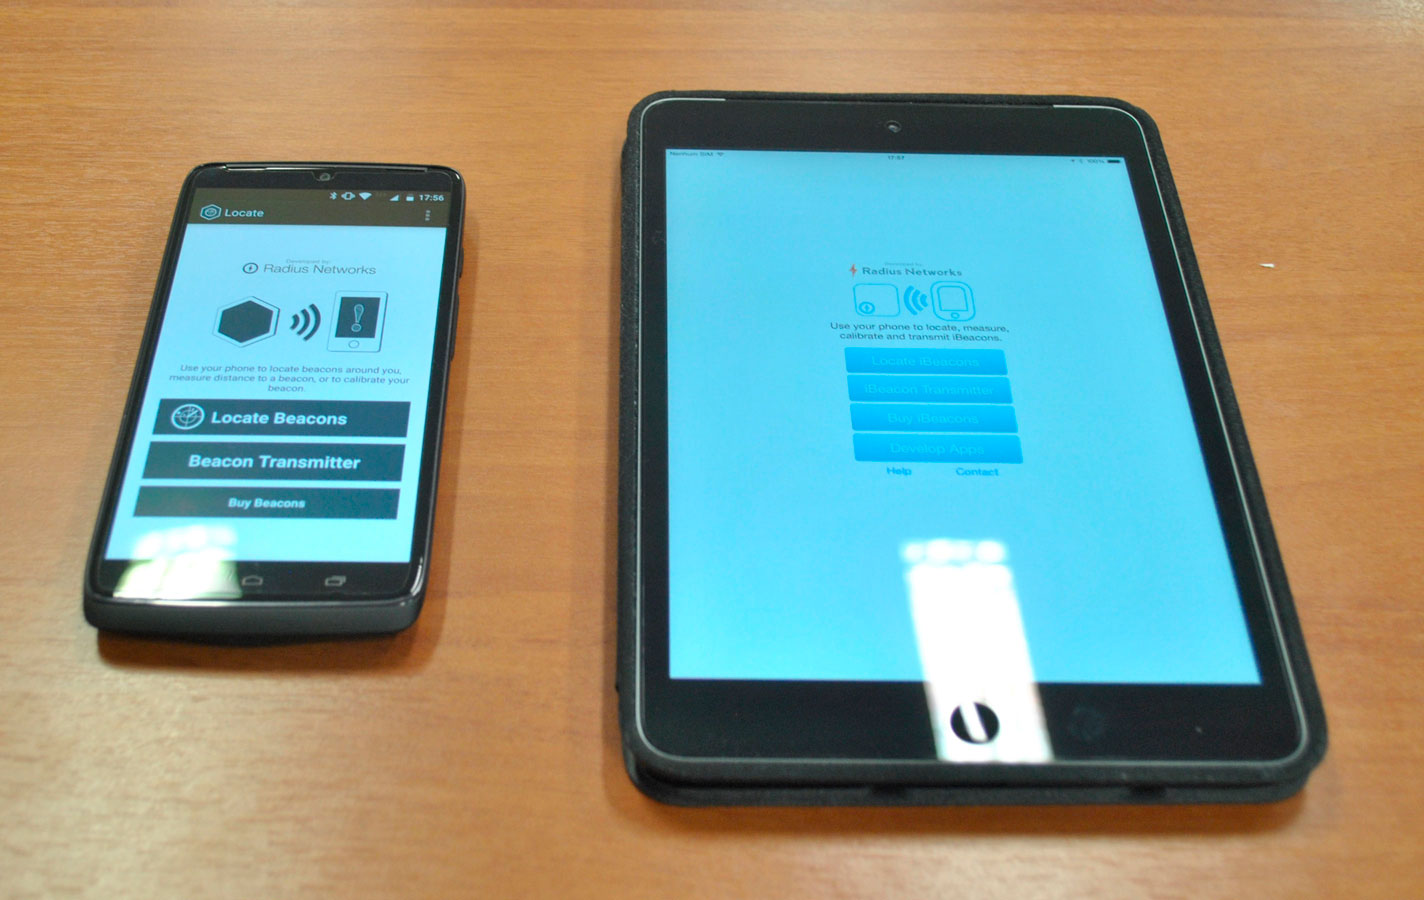
\includegraphics[width=0.8\textwidth]{img/motomaxx-ipad.jpg}
	\end{center}
	\legend{Fonte: elaborado pelo autor}
\end{figure}

% ---
\subsection{\textit{Beacons}}\label{sec:beacons-modo}
% ---

O \textit{beacon} utilizado para testes foi o \textit{Zebra MPact}, conforme \autoref{fig:zebra-mpact}, que utiliza uma bateria CR2450 para alimentação de energia. 

A empresa \textit{Zebra} tem um sistema de administração e gerenciamento nomeado \textit{MPact Toolbox}, instalado em um servidor com sistema Debian 8.1. Esse sistema foi utilizado neste projeto somente para conhecimento da tecnologia \textit{beacon} e atualização do \textit{firmware}, disponível somente via \textit{Toolbox}. Esse software também apresenta a porcentagem de bateria, conforme \autoref{fig:exemplo-toolbox}. Permite a configuração de vários \textit{beacons} simultaneamente, além de alterar o modo de funcionamento, de \textit{iBeacon} para \textit{MPact}, protocolo criado pela fabricante.

\begin{figure}[htb]
	\label{teste}
	\centering
 	\begin{minipage}{0.40\textwidth}
		\centering
		\caption{\label{fig:zebra-mpact}\textit{Beacon} Zebra MPact utilizado para testes.}
		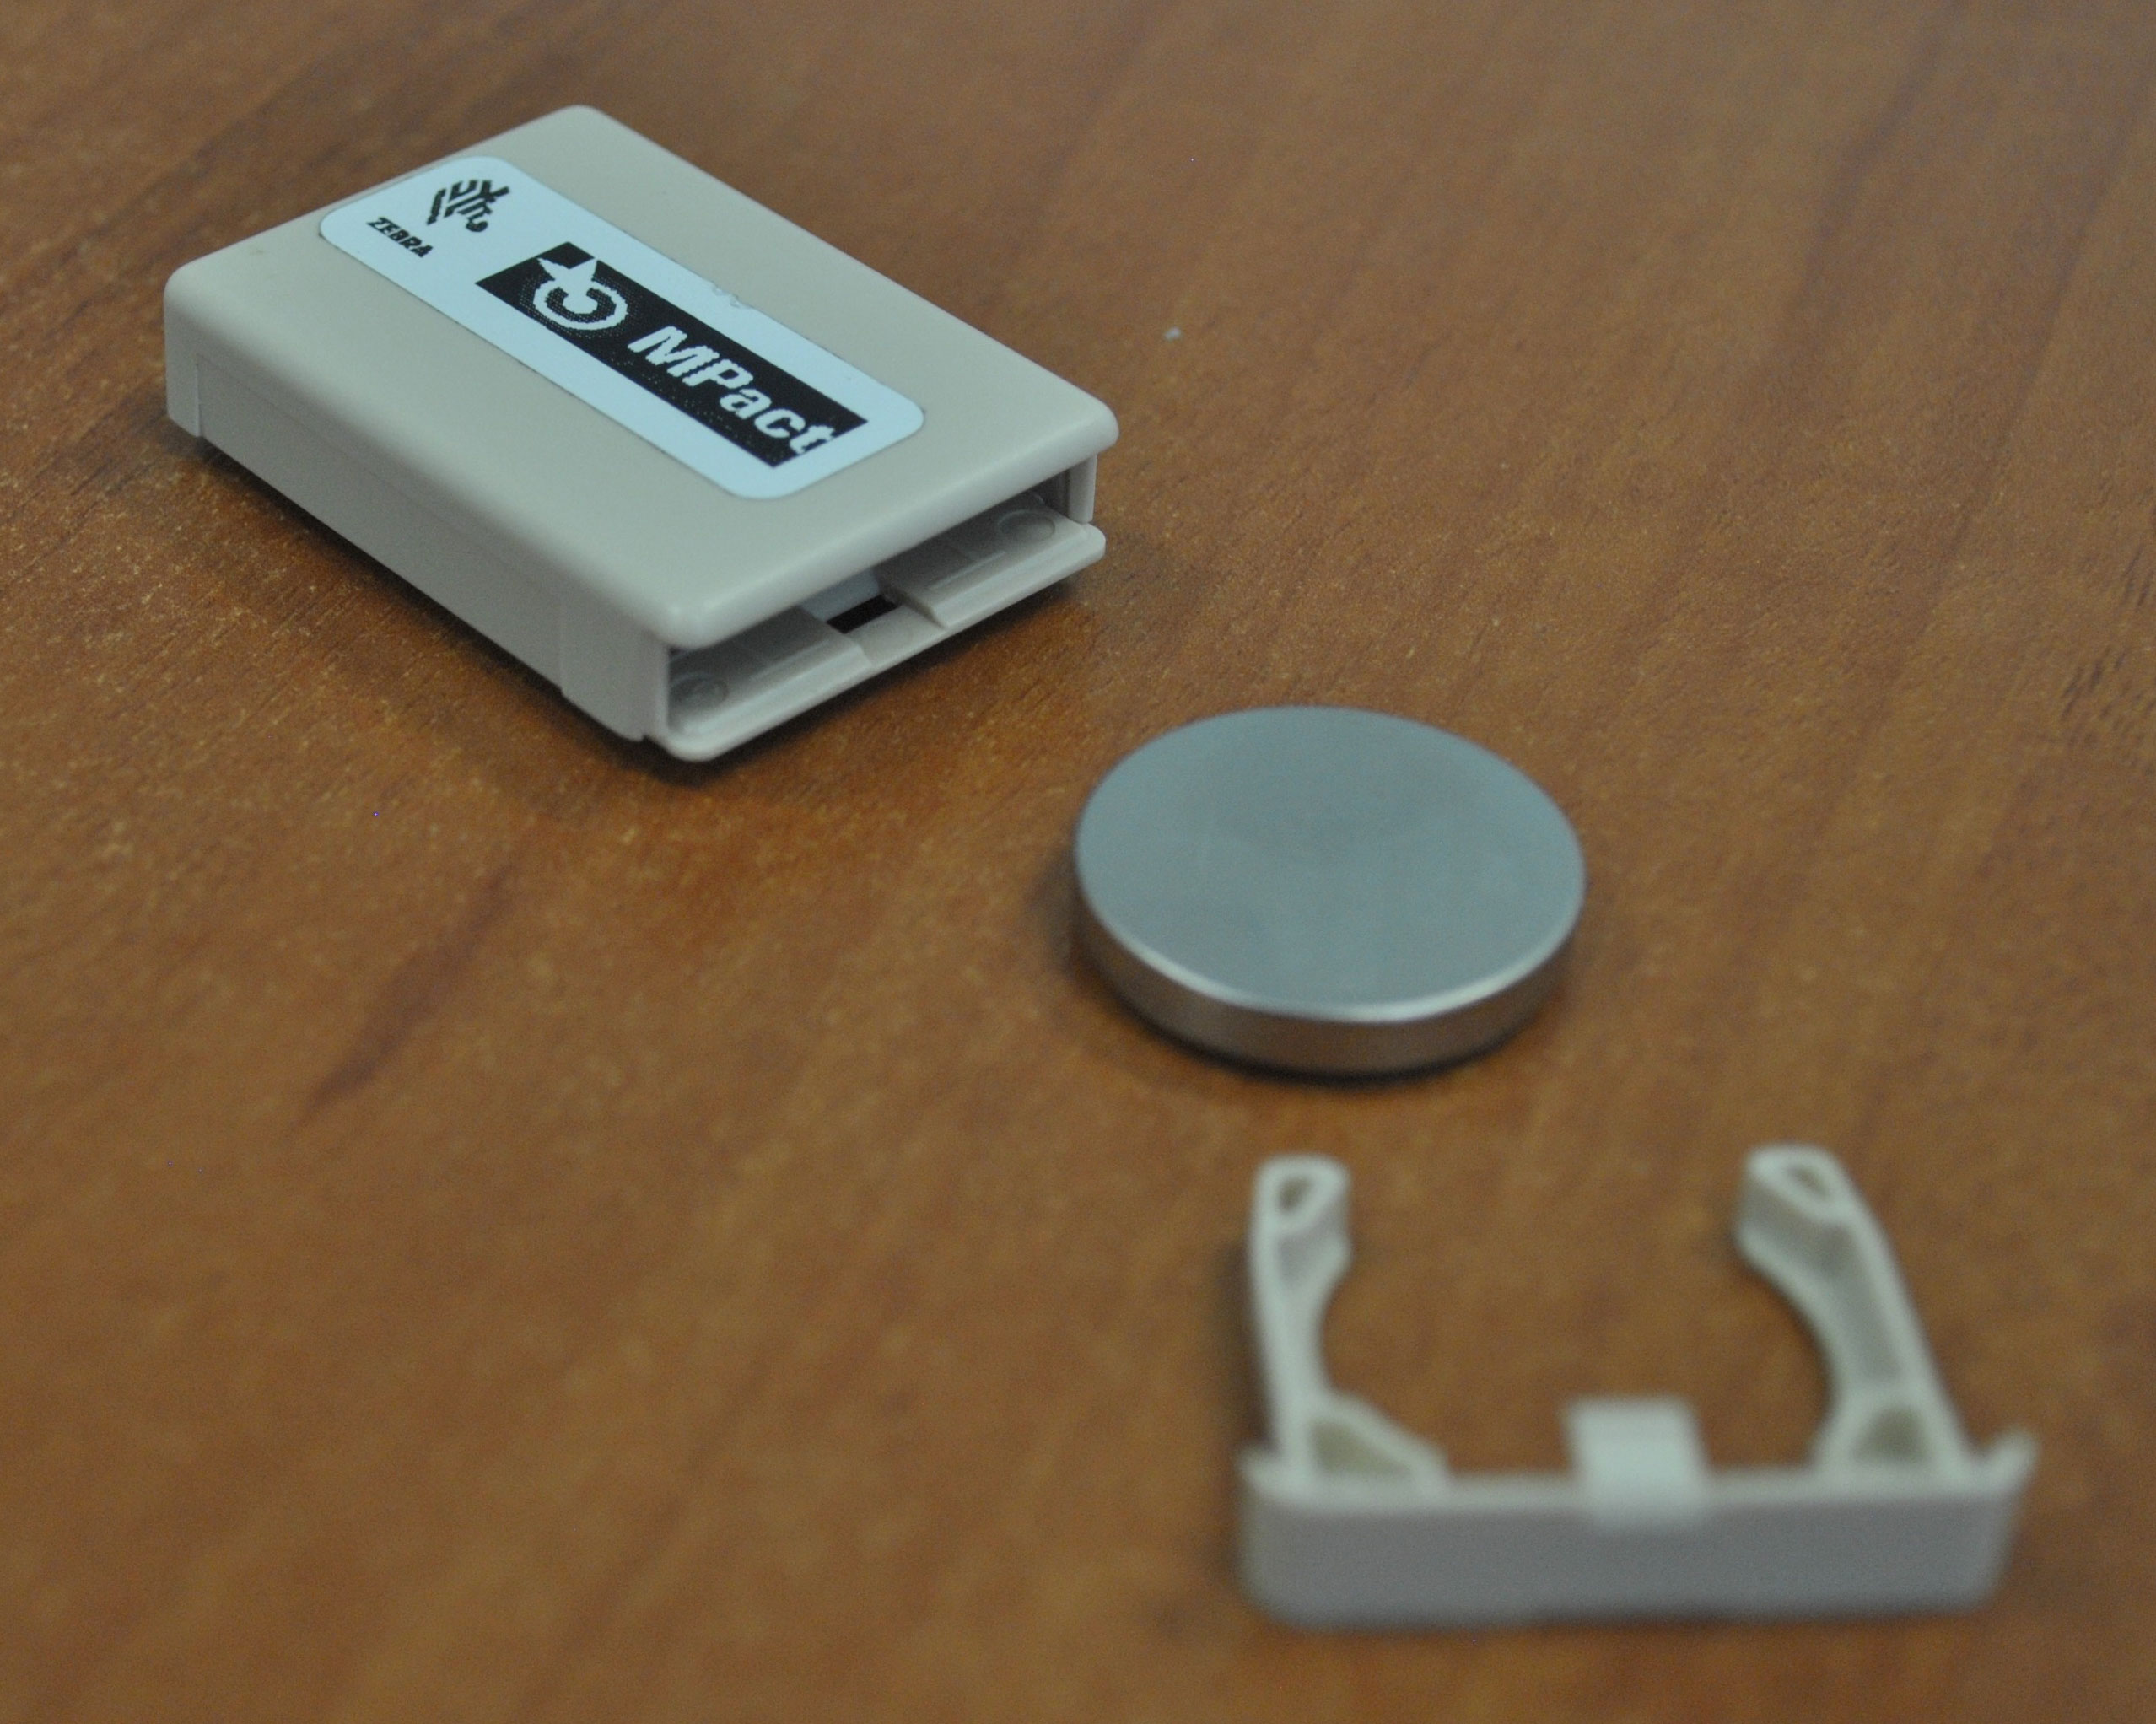
\includegraphics[width=1\textwidth]{img/beacon-mpact2.jpg}
		\legend{Fonte: elaborado pelo autor}
	\end{minipage}
	\hfill
	\begin{minipage}{0.47\textwidth}
		\centering
		\caption{\label{fig:exemplo-toolbox}\textit{Beacon} configurado na \textit{Toolbox} apresentando a porcentagem de bateria.}
		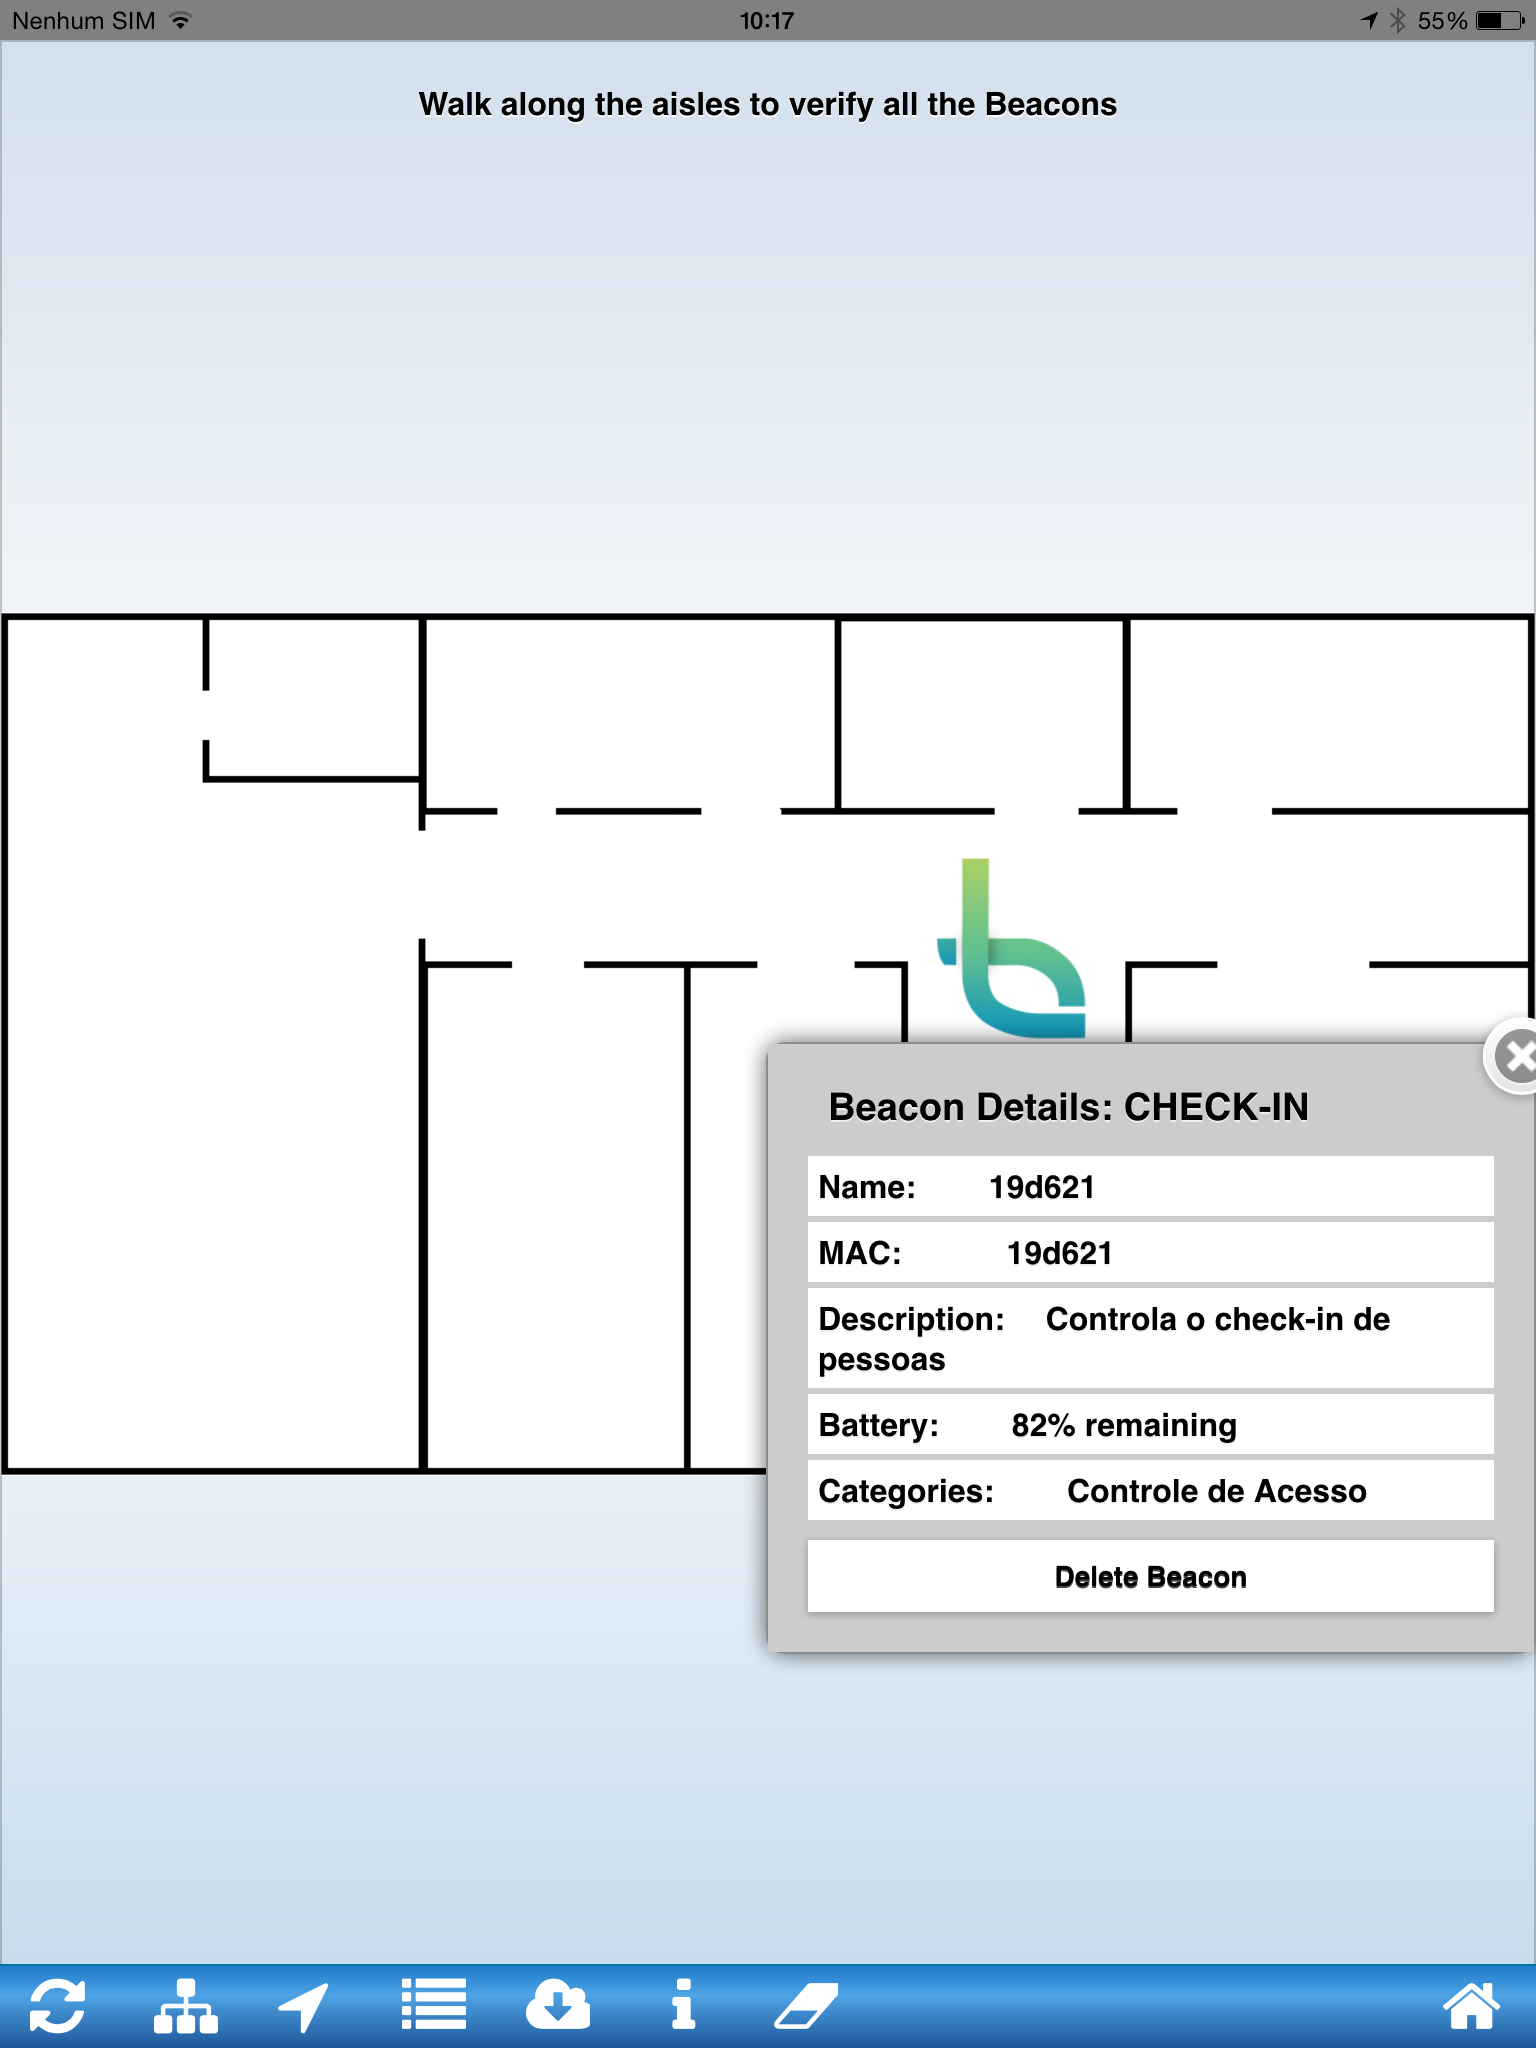
\includegraphics[width=0.9\textwidth]{img/toolbox-exemplo.png}
		\legend{Fonte: elaborado pelo autor}
	\end{minipage}
\end{figure}

% ---
\subsection{Acessórios para o Desenvolvimento do Peacon}\label{sec:acess-prototipo}
% ---

O Peacon foi adaptado em uma caixa de metal (\autoref{fig:caixa-metal}), furada conforme projeto e pintada de preto. Esse processo está detalhado na \autoref{sec:segunda-etapa}. 

\begin{figure}[htb]
	\caption{\label{fig:caixa-metal}Caixa de metal utilizada para o Peacon}
	\begin{center}
		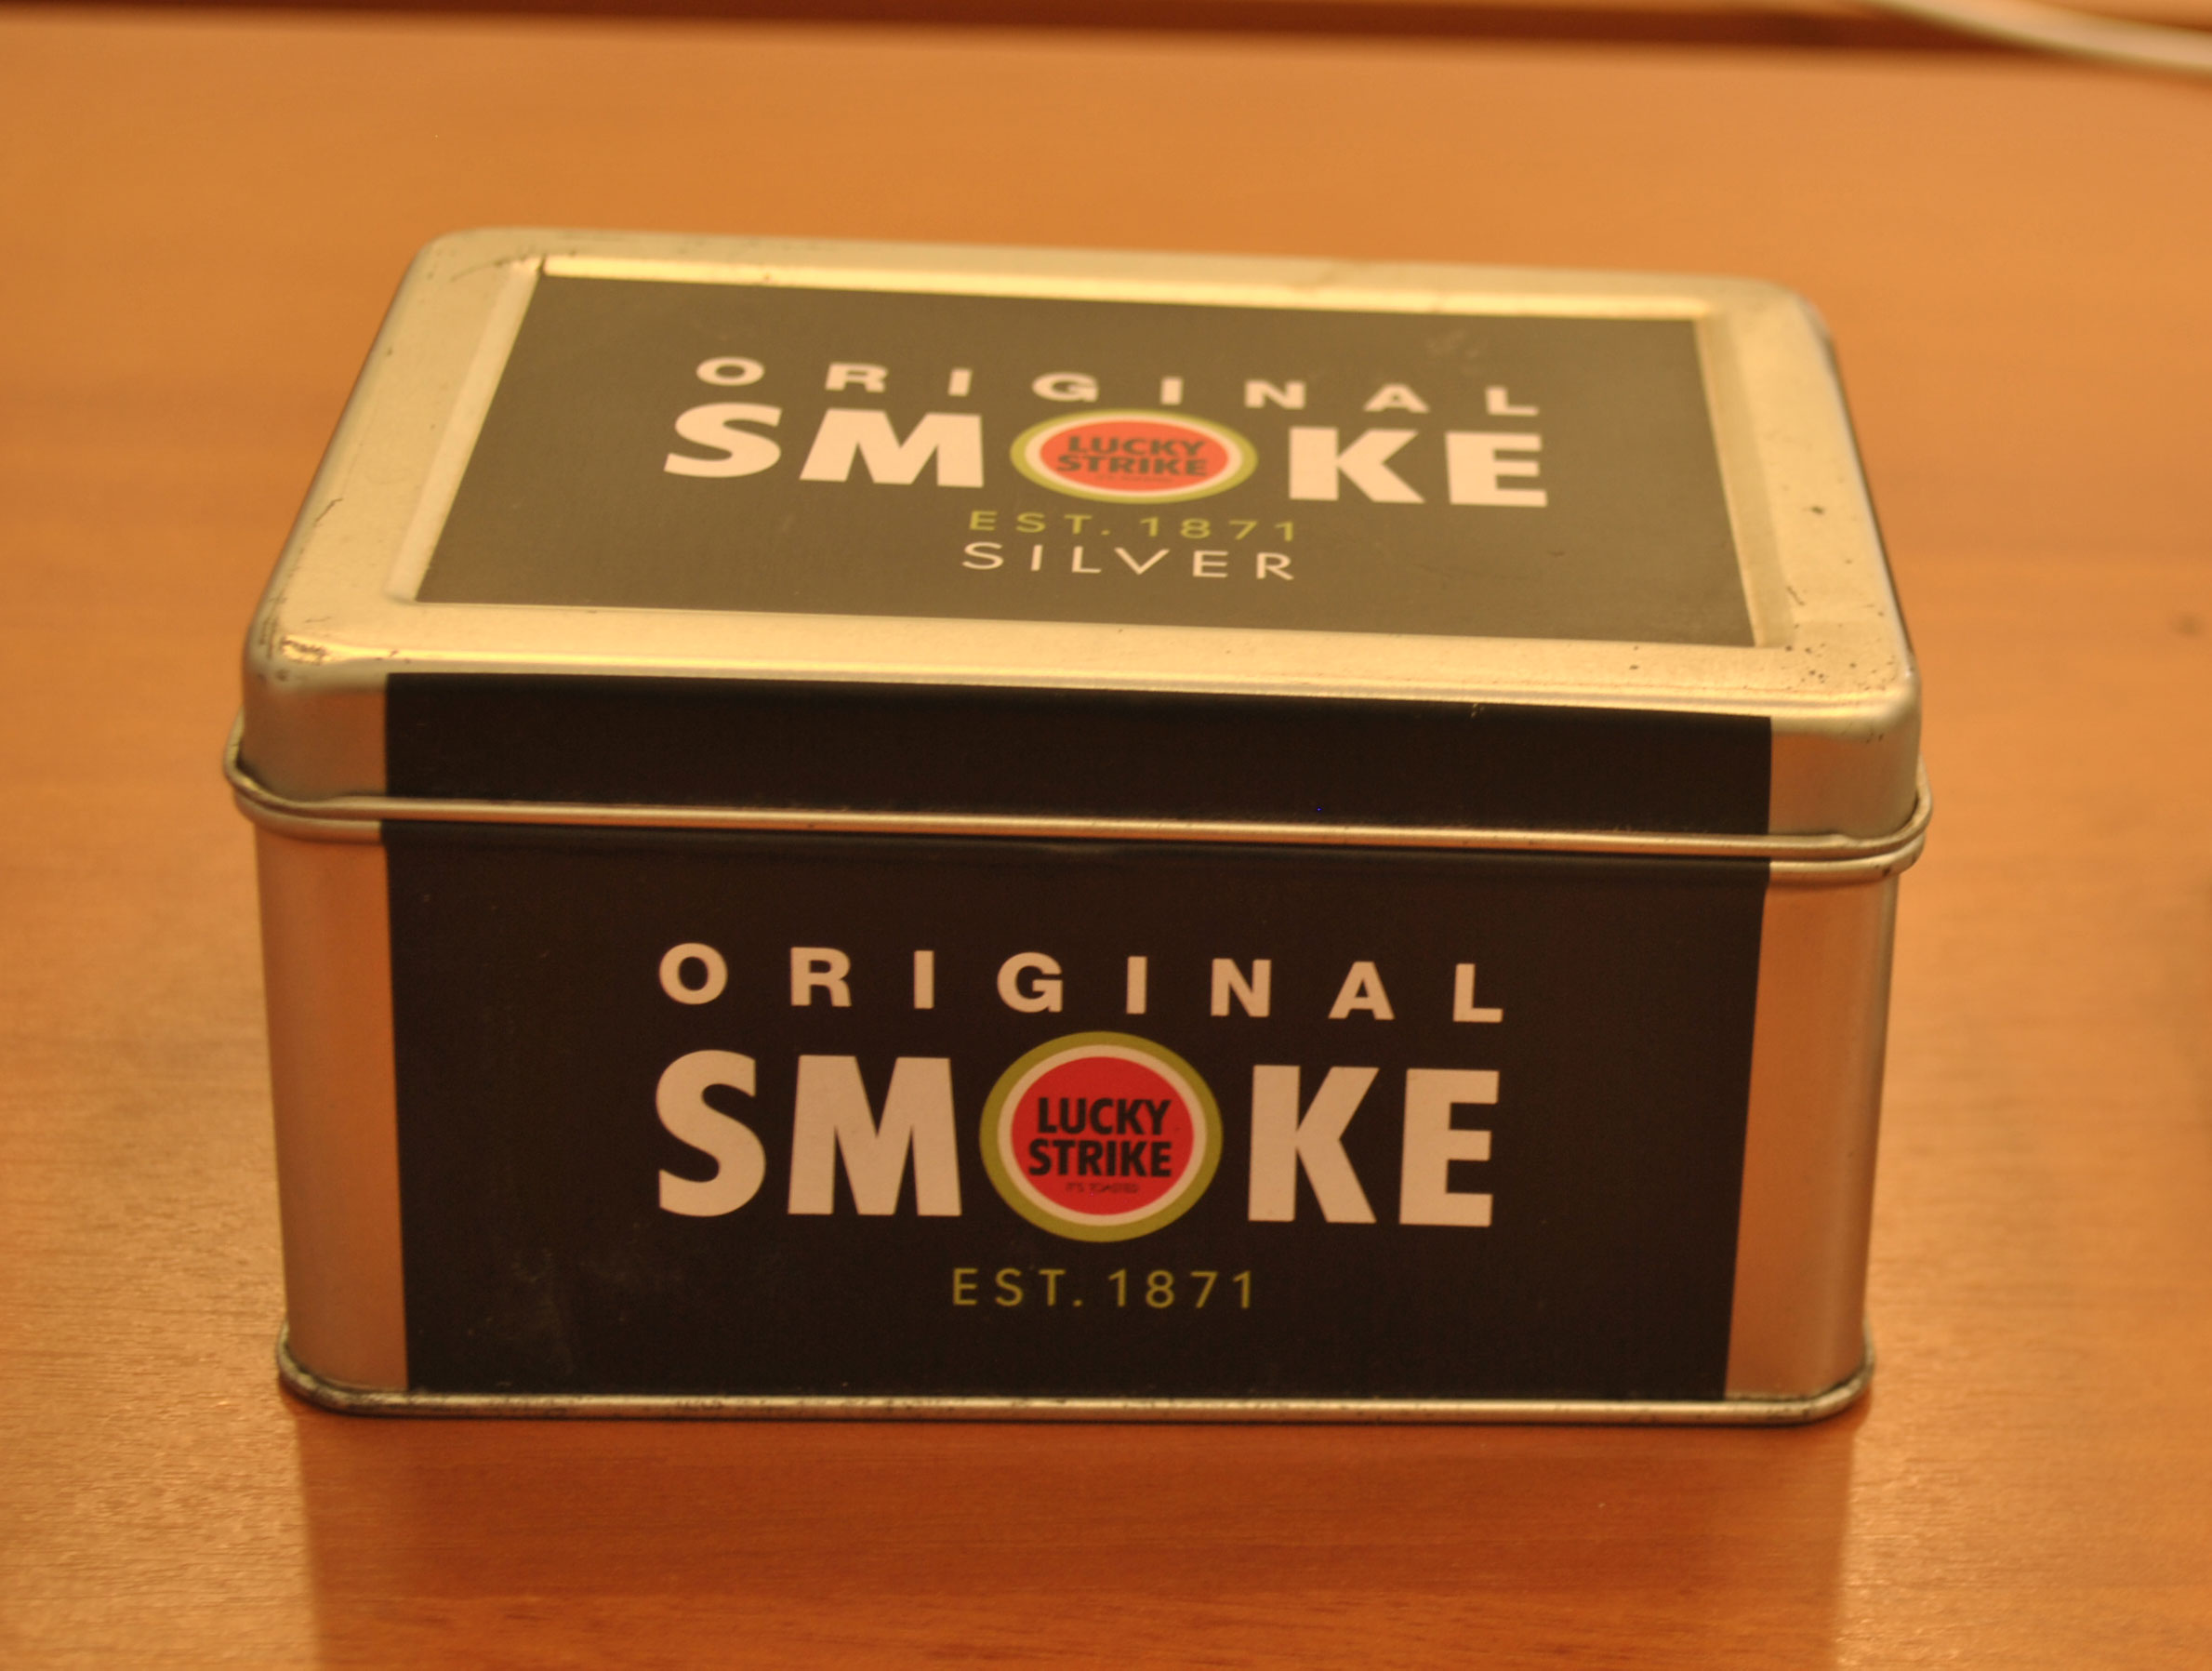
\includegraphics[width=0.5\textwidth]{img/caixa-metal.jpg}
	\end{center}
	\legend{Fonte: elaborado pelo autor}
\end{figure}

Foram utilizados seis LEDs, três resistores de 10K$\Omega$, seis resistores de 330$\Omega$, duas barras de 20 pinos, um display azul de 16 colunas por 2 linhas, três botões do tipo clique, cabos \textit{flat} do tipo IDE e \textit{floppy}, placas com furação para soldagem de componentes, cabos finos removidos de um cabo de rede \textit{ethernet} para ligações entre os componentes e cola quente para fixação dos componentes internos. Esses materiais podem ser vistos na \autoref{fig:prot-interno}.

\begin{figure}[htb]
	\label{teste}
	\centering
 	\begin{minipage}{0.43\textwidth}
		\centering
		\caption{\label{fig:prot-interno}Parte interna do hardware do Peacon}
		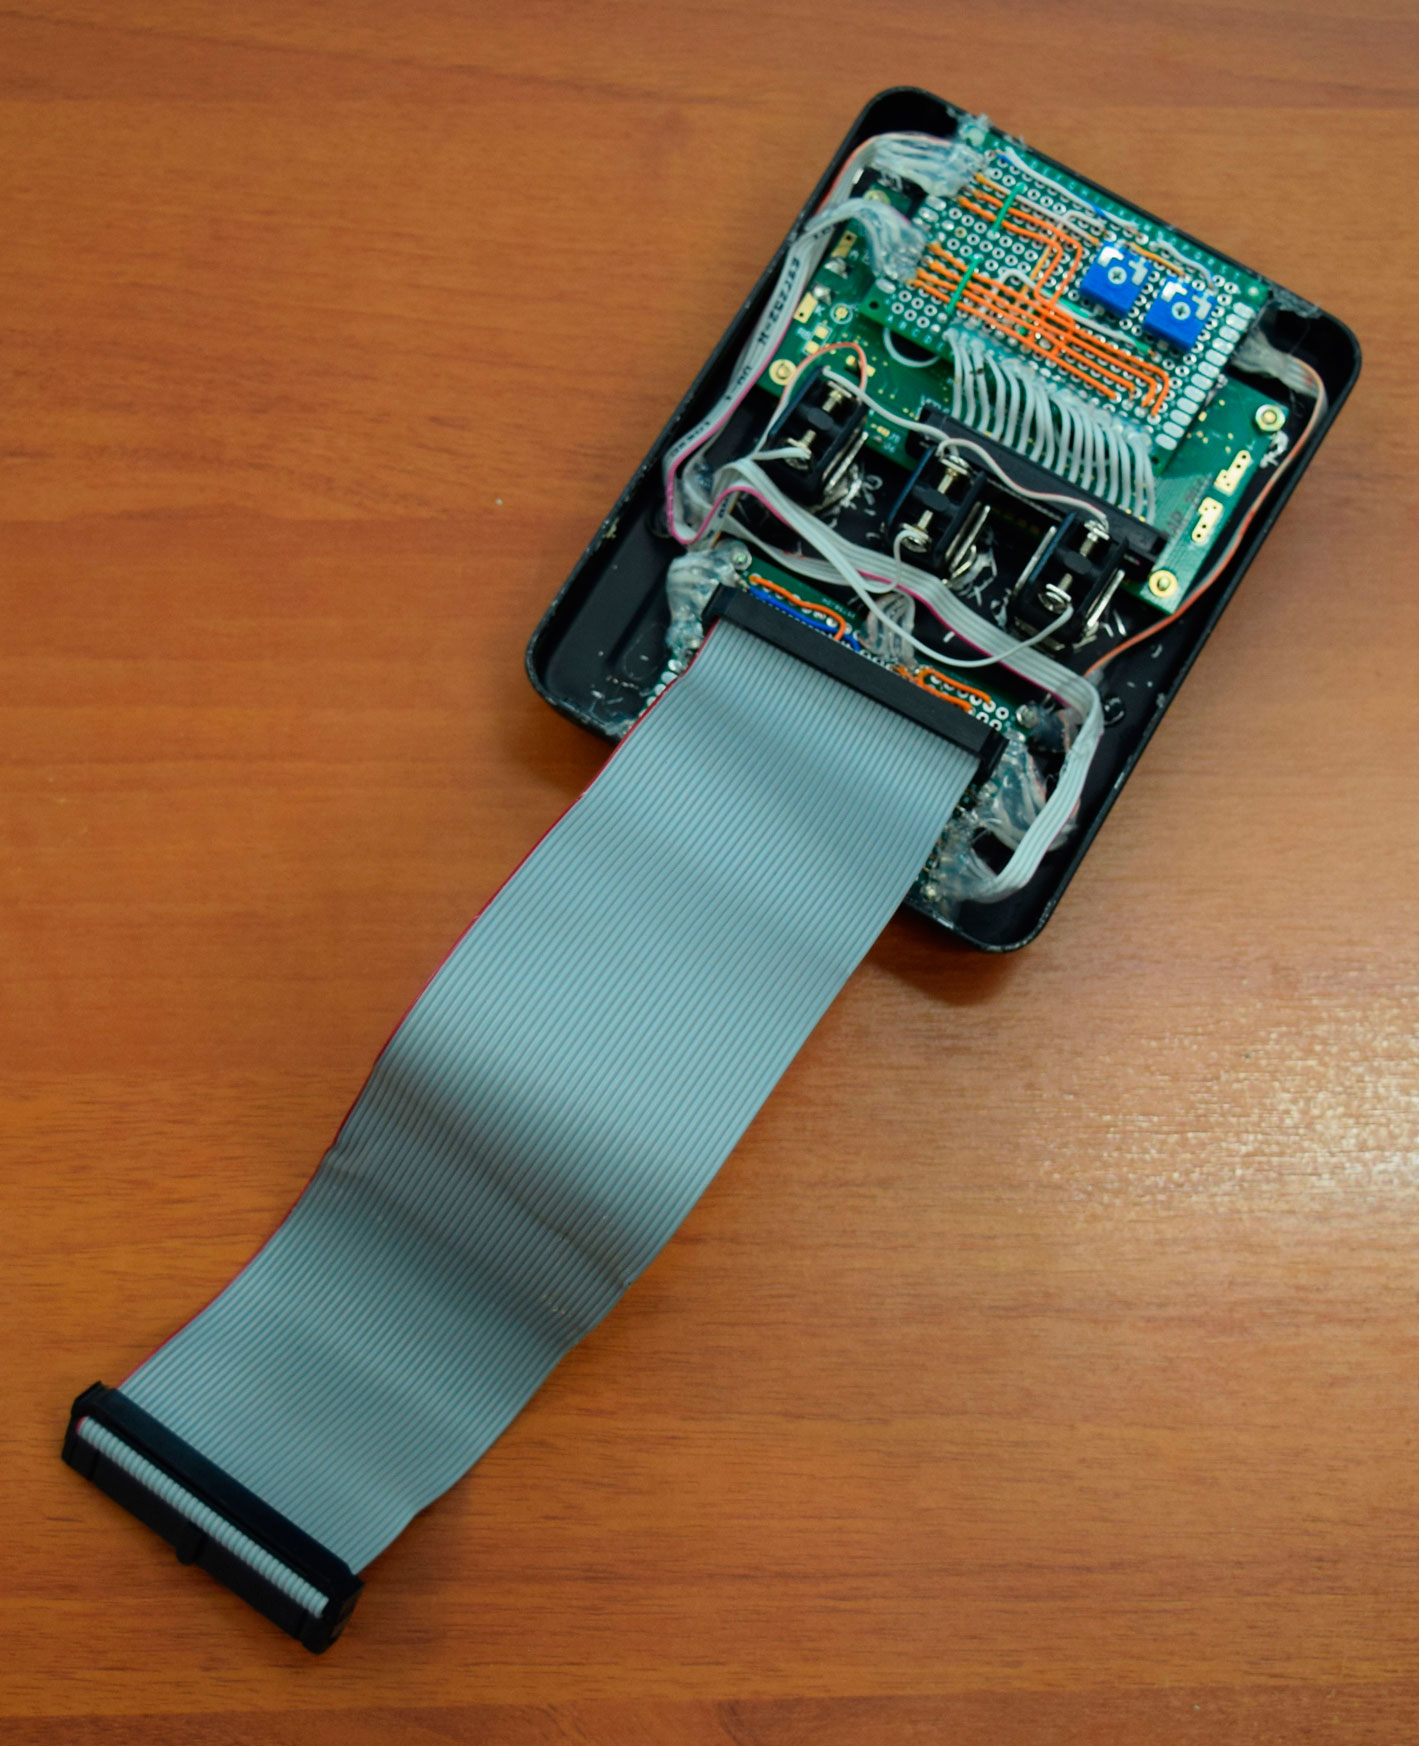
\includegraphics[width=0.7\textwidth]{img/prot-interno.jpg}
		\legend{Fonte: elaborado pelo autor}
	\end{minipage}
	\hfill
	\begin{minipage}{0.55\textwidth}
		\centering
		\caption{\label{fig:proto-teste}Protoboard na etapa de estudo}
		\includegraphics[width=1\textwidth]{img/proto-teste.jpg}
		\legend{Fonte: elaborado pelo autor}
	\end{minipage}
\end{figure}

Durante a fase de estudo das tecnologias utilizou-se uma protoboard e fios de conexão (\autoref{fig:proto-teste}) para testes de código, modo de conexão, entre outros, detalhado na \autoref{sec:segunda-etapa}.

Como o \textit{RPi} tem limitações quanto a quantidade de pinos de entrada e saída digitais (explicados na \autoref{sec:rpi-tecnologia}), os componentes definidos para o protótipo foram determinados conforme possibilidade de conexões. Cada componente necessita de:

\begin{alineas}
	\item um pino de saída digital (GPIO) para acender ou apagar cada LED;
	\item um pino de entrada digital para leitura do estado de cada botão;
	\item seis pinos de saída no total, sendo quatro de dados, um \textit{enable} (ou ativar), e outro \textit{register select}, para o display LCD.
\end{alineas}

O uso desses componentes foram determinados na segunda etapa, detalhada na \autoref{sec:segunda-etapa} - \nameref{sec:segunda-etapa}.


% ----------------------------------------------------------
\section{Tecnologias e Ferramentas Utilizadas}\label{sec:tecnologias-ferramentas}
% ----------------------------------------------------------


% ---
\subsection{Raspberry Pi}\label{sec:rpi-tecnologia}
% ---

O \textit{RPi} é a tecnologia mais importante desse projeto. Já foi abordado na \autoref{sec:raspberry-pi} e \autoref{sec:rpi-acessorios}, porém nessa subseção outros aspectos serão abordados.

A arquitetura da CPU do \textit{RPi 2 modelo B}, utilizado nesse projeto, é baseada na \textit{arm-v7}. Consequentemente todos os softwares devem ser compilados em \textit{arm} para que possam ser executados com sucesso. 

Alguns softwares foram selecionados para utilização, porém não haviam versões \textit{arm} compatíveis ou estáveis para utilização. Entre eles, o banco de dados MongoDB foi descartado pela versão de instalação \textit{arm} não ter sido testada no \textit{RPi}, e gerada pela comunidade. Diversos relatos de \textit{bugs}, mal funcionamentos e incompatibilidade levaram a mudar a tecnologia de banco de dados.

Uma ferramenta muito importante disponível no \textit{Raspberry Pi} são as GPIOs, ou \textit{General Purpose Input/Output} - portas de entrada e saída de uso geral (\autoref{fig:gpio-pins-pi2}).  

\begin{citacao}
"Esses pinos são a interface física de conexão entre o Pi e o mundo. No mais baixo nível, você pode pensar desses pinos como interruptores que você pode ligar ou desligar (entrada) ou que o Pi possa ligar ou desligar (saída). Dos 40 pinos, 26 são pinos de GPIO e os outros são pinos de energia ou terra.". \cite{rpi-gpio}
\end{citacao}

Seguem um padrão definido de numeração (\autoref{fig:gpio-numbers-pi2}). Esses números são utilizados diretamente na programação para acessar os pinos e interagir com o que estiver conectado ali.

\begin{figure}[htb]
	\caption{\label{fig:gpio-pins-pi2}Pinos físicos de conexão}
	\begin{center}
		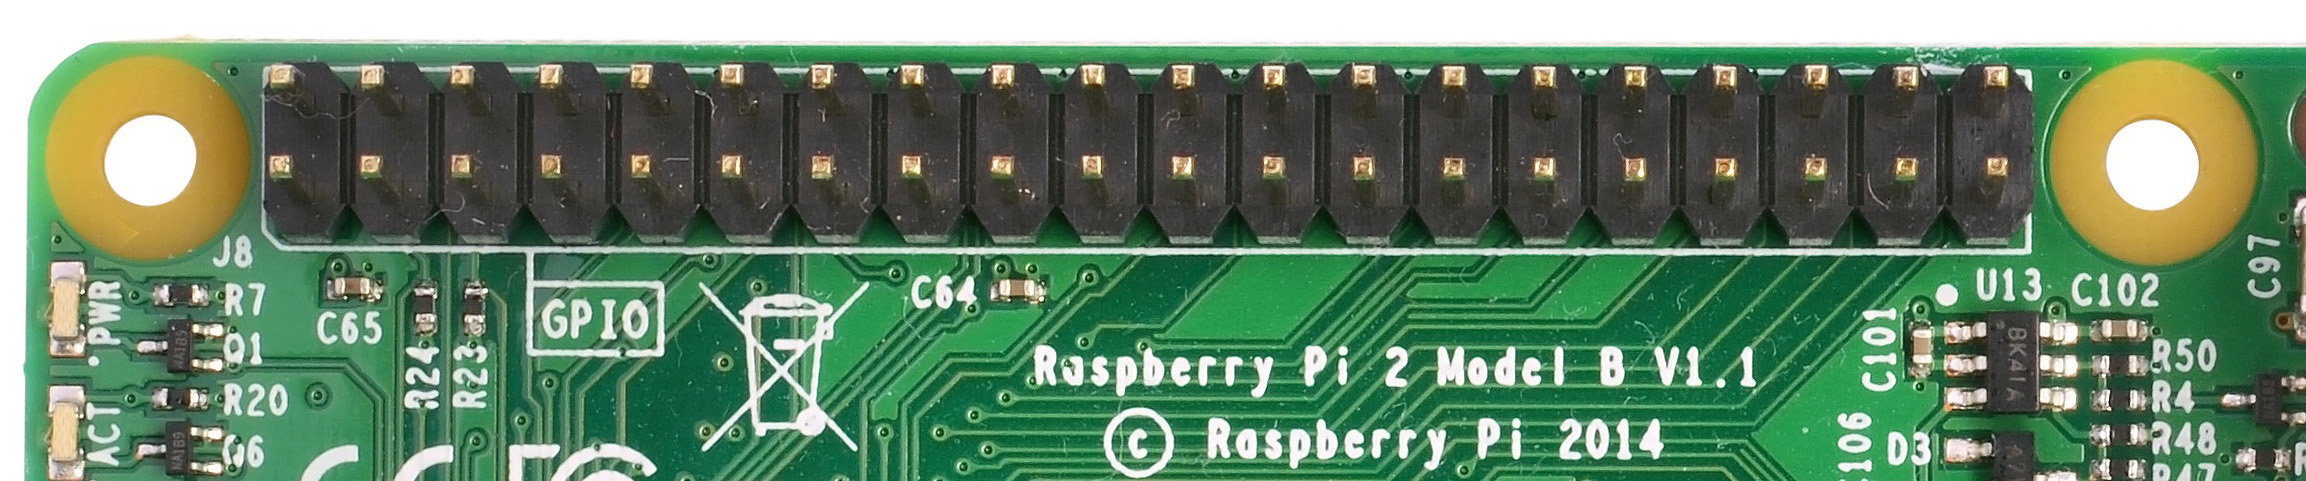
\includegraphics[width=0.8\textwidth]{img/gpio-pins-pi2.jpg}
	\end{center}
	\legend{Fonte: \cite{rpi-gpio}}
\end{figure}

\begin{figure}[htb]
	\caption{\label{fig:gpio-numbers-pi2}Numeração dos pinos de conexão}
	\begin{center}
		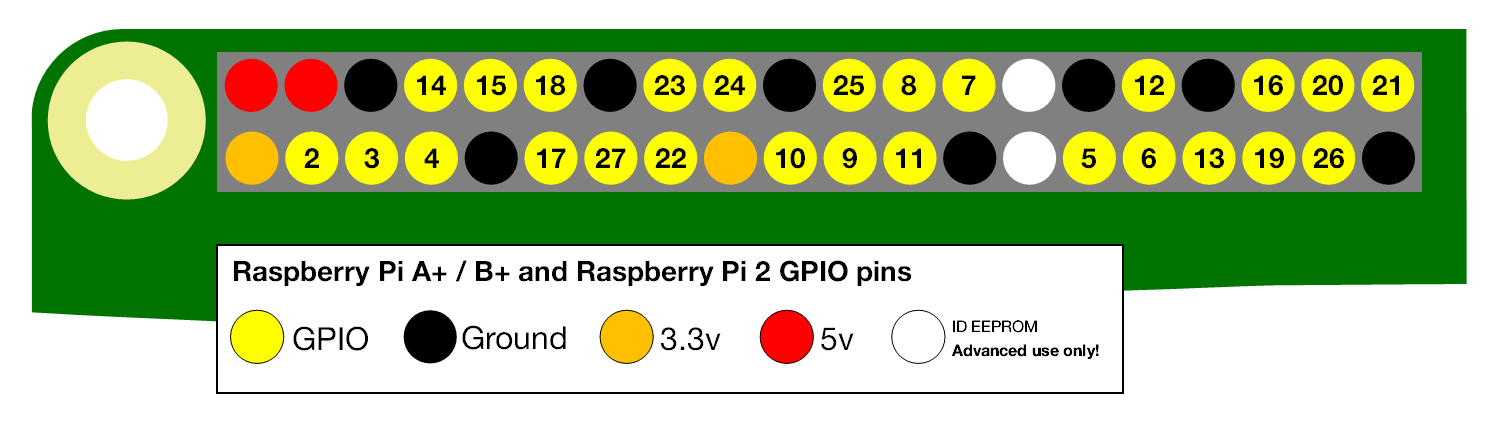
\includegraphics[width=0.8\textwidth]{img/gpio-numbers-pi2.png}
	\end{center}
	\legend{Fonte: \cite{rpi-gpio}}
\end{figure}


% ---
\subsection{Node.js e npm}\label{sec:node-js}
% ---

Node.js\footnote{\url{https://nodejs.org/}} é uma plataforma de aplicações baseada no motor de Javascript do Google Chrome chamado V8. \cite{o-que-e-node}. A linguagem Javascript normalmente é utilizada no navegador, no chamado lado do cliente, porém o Node leva essa linguagem de programação diretamente para o sistema operacional, permitindo que aplicações sejam executadas direto no lado servidor. Seu código fonte está disponível\footnote{\url{https://github.com/nodejs/node}} para acesso, colaboração e comentários.

Utiliza um modelo de aplicações voltado a eventos, ou seja, não bloqueia a execução do código com entrada e saída, cálculos, etc. Em vez disso dispara as funções quando os eventos forem acionados. \cite{o-que-e-node}.

Essa plataforma possui um aplicativo chamado \textit{Node Package Manager} (denominado \textit{npm}). Esse aplicativo auxilia a instalação e distribuição de pacotes e bibliotecas auxiliares, normalmente criadas pela comunidade e de código livre. Qualquer pessoa pode criar sua biblioteca, enviar ao GitHub, e enviar ao \textit{npm}.

O \textit{npm} cria o arquivo \textit{packages.json} e salva todas as informações do projeto. Nome do projeto, do criador, link para o repositório no GitHub, dependências de bibliotecas com a versão específica instalada, entre outros. Facilita o trabalho de outra pessoa, pois quando utilizar o código fonte, executando o comando \textit{npm install} o mesmo baixa e instala todas as dependências para executar aquele aplicativo.

Diversos pacotes foram utilizados no desenvolvimento desse projeto:

\begin{alineas}
	\item \textbf{\textit{bleacon}}: para descoberta e transmissão de pacotes \textit{beacon};
	\item \textbf{\textit{lcd}}: auxilia na conexão com displays de LCD;
	\item \textbf{\textit{nano}}: auxilia na conexão com o banco de dados CouchDB;
	\item \textbf{\textit{onoff}}: disponibiliza funções para conexões com LEDs, botões e hardwares no geral - específico para Raspberry Pi e BeagleBone\footnote{Computador do tamanho de um cartão de crédito, similar ao Raspberry Pi};
	\item \textbf{\textit{node-constants}}: facilita o uso de constantes entre arquivos e funções;
	\item \textbf{\textit{numeral}}: funções para manipulação avançada de números inteiros e floats;
	\item \textbf{\textit{is-online}}: função para validar conexão com a internet;
	\item \textbf{\textit{internal-ip}}: função para retornar o endereço de IP da rede interna;
	\item \textbf{\textit{public-ip}}: função para retornar o endereço de IP da rede externa, ou IP público.
\end{alineas}

Quando foi instalado no Raspbian Wheezy, a versão mais recente compatível e recomendada para o \textit{RPi} era a v0.12.6. Atualmente já existem versões mais novas, porém essa versão permaneceu por questões de compatibilidade com o software desenvolvido.

Para que o sistema executasse constantemente e automaticamente toda vez que o \textit{RPi} fosse ligado, um software desenvolvido em Node.js foi utilizado, denominado pm2\footnote{\url{https://github.com/Unitech/pm2}}. Esse aplicativo permite iniciar um software desenvolvido em Node.js, fornece ferramentas para monitorar, reiniciar, parar, entre outras funcionalidades.

% ---
\subsection{CouchDB}\label{sec:couchdb}
% ---

CouchDB\footnote{\url{http://couchdb.org/}} é um sistema gerenciador de banco (SGBD) de dados voltado para a \textit{web} e \textit{apps mobile}. Não é um SGBD baseado em SQL, em vez disso utiliza documentos no formato \textit{JSON} (JavaScript Object Notation)\footnote{Modo de formatação dos dados muito leve, utilizado para troca de informações entre máquinas, por ser de fácil interpretação e geração. \cite{json-couch}.}, as conexões e requisições são feitas por HTTP (similar a uma conexão a um site), além de permitir servir páginas web direto do banco de dados.

Esse sistema foi utilizado neste projeto pela facilidade de uso com o Node.js. O pacote \textit{nano} para Node abstrai toda a conexão com o banco de dados, permitindo que pouco código seja utilizado. Os documentos gerados no formato JSON no Javascript são enviados diretamente ao CouchDB sem necessidade de tratamento, manipulação ou configuração.

Disponibiliza uma ferramenta web para acesso aos bancos de dados criados denominada \textit{Futon}, a partir da instalação já funciona normalmente acessando o endereço \textit{http://localhost:5984/\_utils/} (\autoref{fig:futon-overview}).

\begin{figure}[htb]
	\caption{\label{fig:futon-overview}Futon - manipulação dos bancos de dados CouchDB}
	\begin{center}
		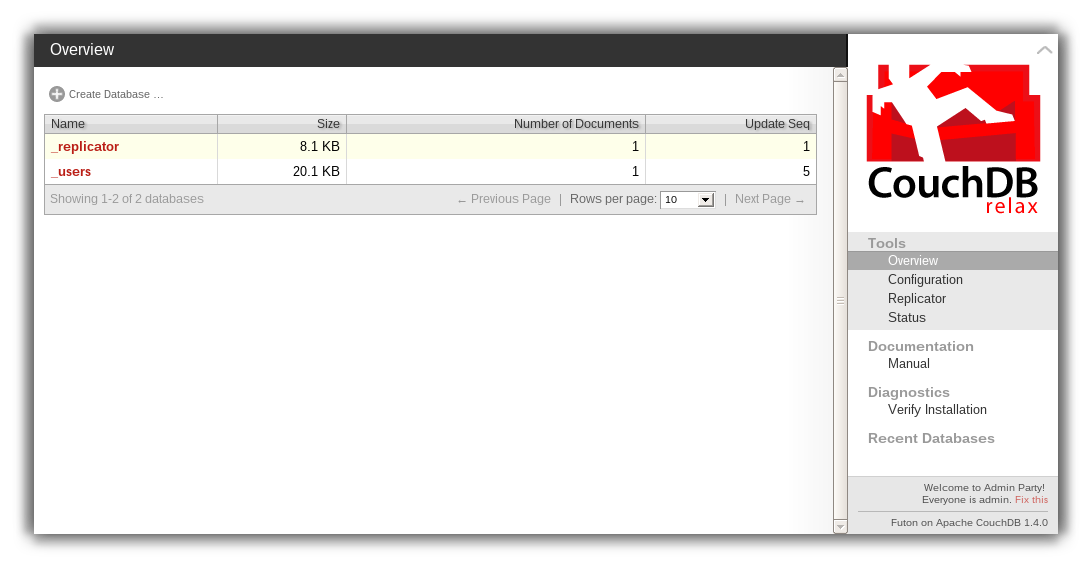
\includegraphics[width=0.75\textwidth]{img/futon-overview.png}
	\end{center}
	\legend{Fonte: \cite{futon-couch}}
\end{figure}

% ---
\subsection{Git}\label{sec:git}
% ---

Git é um software de controle de versão para repositórios. Registra as mudanças nos arquivos (ou grupo de arquivos) ao longo do tempo, de forma que as versões possam ser recuperadas futuramente. \cite{pro-git}. Caso necessário voltar algumas versões por \textit{bug} no código, mal funcionamento de uma função recém implementada ou outras razões, as alterações estarão documentadas.

Atualmente o Git é muito utilizado por projetos de código aberto, como por exemplo o Swift\footnote{\url{https://github.com/apple/swift}} que é uma linguagem de programação criada pela Apple voltada para seus sistemas operacionais, e o AngularJS\footnote{\url{https://github.com/angular/angular.js}}, framework Javascript mantido pelo Google.

É possível configurar o repositório local para sincronizar com um repositório remoto, por meio de \textit{push} (enviar mudanças) e \textit{pull} (buscar mudanças). Dessa forma promove a divisão do trabalho, removendo o problema de sincronização de código entre diferentes máquinas e usuários.


% ----------------------------------------------------------